
\begin{abstract}
Despite the recent improvements in admissible heuristic search techniques
in classical planning, it is known that the the exponential growth of
search plateau in A* is unavoidable even under the optimistic assumption.
 % 
We investigate various existing myth on tiebreaking
strategies and propose simple yet effective methods for improving the
search performance within plateau.
 % 
 % 
 They do not depend on any particular heuristic, nor
 on multi-heuristic portfolio.
 They work even if the heuristic
 function no longer provides useful information.
 % Moreover, they do not even try to obtain any further information from
 % the domain.
 We empirically evaluate our strategies against state-of-the-art admissible planner.
\end{abstract}

Since the advent of delete-relaxation and abstraction heuristics in
admissible Classical Planning, much of the interest was focused on improving
the accuracy of these heuristic functions to prune more nodes from the
search space.
% 
However, recent work by Helmert and Roger
\shortcite{helmert2008good} claims that, even with an optimistic
assumption of \emph{almost-perfect heuristics}, \astar still has an
exponentially large plateau. They conclude that the further performance
improvement requires the techniques orthogonal to the heuristic
function, such as symmetry breaking, domain reduction, factored planning
etc.

In this paper, we focus on the tiebreaking criteria of \astar.
Sophisticated tiebreaking is a heuristic-agnostic improvement and thus 
falls into above category of techniques.
It trivially maintains admissibility because it works only within the
same f-value and does not alter the expansion order wrto f-value.

% such technique.
% tiebreaking strategy for \astar.
% Our tiebreaking strategies fall into this category.

% The attention to the search algorithm itself is relatively small since
% most literature depends on bare \astar.  This was because variations of
% best first search focus on different requirements, such as IDA* on
% linear space, WA*/Lazy-A*/GBFS/EHC on trading speed for optimality, RWA*
% on replanning, etc., and not on improving upon \astar itself.

% maintaining all of its charactristics: memory-greedy yet efficient
% optimal algorithm.

Specifically, we show several important findings regarding the
existing tiebreaking strategy for \astar as follows.
% 
First, in implementing the open list of \astar, priority queue based on
LIFO-buckets is more efficient than that of FIFO-buckets.
% 
Second, with LIFO-based implementation, $h$-based tiebreaking which
frequently appears in the heuristic search literatures have little
impact on the performance.
% 
Third, the LIFO-based bucket implementation and $h$-based tiebreaking
both share the greedy search pattern within the plateau of the
search space.
% 
Fourth, based on these observations, we propose a tiebreaking
method based on the \emph{depth} within the plateau.
%
Finally, comparison results of different variations of depth-based
strategy showed that they are not dominating each other. Therefore, we
propose a new class of portfolio strategy which alternates between
several tiebreaking methods.
It has a theoretical worst case guarantee that it
never evaluates the nodes any more than $N$ times the \emph{minimum} number
of evaluation required by the best tiebreaking method among $N$ methods
under the portfolio.
Also, it is characteristic in that it works with a single heuristic function.
% 

The rest of paper is organized as follows: The next section describes the
preliminary backgrounds of \astar.
Next we compares several trivially-simple and well-known tiebreaking
methods on top of Fast Downward to show that even such a small
difference significantly affects the performance on domains with
large plateaus.
Next we propose a novel depth-aware tiebreaking methods and empirically
show that it outperforms previous strategies.
Then we proceed to evaluate the tiebreaking portfolio.
We finally conclude with a discussion on the future work.

\section{Backgrounds and Preliminary}
\label{sec-1}

\subsubparagraph{\astar and perfect heuristics}

\astar is one of the mainstream algorithms for finding an optimal path in the
search space represented as a graph, and has been used extensively in
STRIPS planning in the recent years.
\astar stores the search nodes into two priority queues called an
\emph{open list} and a \emph{closed list}. In these queues, the search
nodes are sorted based on $f$ value, which is a sum of the actual cost
$g$ from the initial state and the cost estimate $h$ to the goal
state. $h$ is computed by the heuristic function.
% On each iteration, \astar expands the open nodes with the
% smallest $f$ value and mark them as closed. Its successor nodes are
% accordingly inserted back to the open list or closed list, while
% sometimes the parent node is updated so that it has the shortest path
% from the initial state.

% Due to the space limitation,
% we assume the readers are already familiar with \astar
% and skip the details of the algorithm.

\astar returns an optimal solution when $h$ is admissible, i.e., when it
never overestimate the true distance to the goal $h^*$.
Trivially, the best possible admissible heuristic function is $h^*$ itself, which is
called \emph{perfect heuristics}.
It is known that with a perfect heuristics the planner do not have to
conduct any search: There are no multiple possibilities that the
planner should examine on each node.
However, computing $h^*$ is PSPACE-Complete,
which is as difficult as solving the problem itself and is not
practical.

\emph{Almost perfect} heuristics $h_c$ is a class of similar
impractical, theoretical functions which is also PSPACE-Complete to
compute \cite{helmert2008good}.  It has a constant error $c$ from the
perfect heuristic $h^*$, i.e., $h_c=h^*-c$.  The important finding by
\citeauthor{helmert2008good} is that, even if we assume this intractable and
optimistic heuristic function was obtained, the number of the nodes in the final
plateau of the search space becomes exponentially large as the problem size
increases. Based on this fact, they claimed that relying on the
improvement of the heuristic functions has a limitation,
and the researchers should seek the other, orthorgonal improvements.

\subsubparagraph{\sota heuristics}

These intractable heuristics are of course very hard and expensive to
compute. However, even the practical and tractable \sota heuristic
functions for STRIPS Planning, such as \lmcut\cite{Helmert2009} and
IP-based heuristics[???], are so heavily CPU intensive that they
outweighs the space-greedy nature of \astar. Also, compared to the other
functions, these functions dominate the search time over the other
factors of planning algorithms, such as node insertion and deletion.

In contrast, another class of \sota heuristic functions called abstraction-based heuristics
such as PDB \cite{edelkamp2001planning} and M\&S \cite{helmert2007flexible}
are known to allow for faster node expansion while providing a good estimate.
However, they tend to consume large amount of preprocessing time and also
the large amount of memory to constract and maintain the abstraction
space,
and the performance tends to be memory-bounded rather than CPU-bounded,
which is also doubled by the fast expansion.

\subsection{Tiebreaking Strategies in \astar}

Aside from the heuristic function, most best-first family of search
algorithms, including \astar, IDA* and so on, have a tiebreaking criteria which is used
when two nodes have the same $f$ value.
There are two mainstreams of tiebreaking criteria in these algorithms:
$h$-based tiebreaking and LIFO-tiebreaking.

The original \astar paper \cite{hart1968formal} explains the default
tiebreaking in \astar as ``always in favor of any node $n \in T$ [goal
node]'', implying that it break ties by choosing the nodes which are
nearer to the goal, which means larger $g$ and smaller $h$.
\citeauthor{Korf1985depth} uses $h$-based tiebreaking in the context of WA*
\cite{korf1993linear}.  \citeauthor{hansen2007anytime} claim it is
``well-known that \astar achieves best performance when it breaks ties
in favor of nodes with least h-cost'' \cite{hansen2007anytime}, and
\citeauthor{holte2010common} also writes ``\astar breaks ties in favour
of larger g values, as is most often done'' \cite{holte2010common}.
\citeauthor{felner2011inconsistent} also assume ``ties are broken in
favor of low h-values'' in describing Bidirectional Pathmax for \astar.
\citeauthor{burns2012implementing} also break ties ``preferring high
g'', which means low $h$. They also writes ``The reasoning is that the
goal can be found more quickly in the final $f$ layer of search''. We
assume this is a consensus among the researcher of forward heuristic
search, but this is not extensively tested yet.

Analysis on LIFO-based tiebreaking is not as abundant as in $h$-based
tiebreaking and is largely forgotten.
\citeauthor{Korf1985depth} assumes LIFO ordering in describing \astar,
as ``\astar employes the tie-breaking rule of 'most
recently generated''' \cite{Korf1985depth}.
\citeauthor{burns2012implementing} did not mention anything about how
the bucket of nodes with the same $h$-value is implemented, but from their
open-sourced implementation, they use LIFO for second-level tiebreaking. 
In contrast, current implementation of \sota \astar based planner Fast
Downward \cite{Helmert2006} uses FIFO-queue for implementing the bucket
of $h$-based tiebreaking, again giving no explanation to this decision.

Another related techinques are found in the context of satisficing planning.
An inadmissible search technique in LAMA planner \cite{richter2010lama}
increases every action costs by 1, called \emph{PLUSONE} cost-type.
It is explicitly targeted at zero-cost actions observed in Openstacks,
and resulted in a significantly better performance in IPC-6.
In PLUSONE, three successive
applications of zero-cost operators result in cost 3, and two
applications result in a cost 2, and smaller cost is preferred, just as
\astar always expands the node with smaller $f$-value.
Another technique in LAMA is \emph{preferred operator queue},
which is a technique that favors those actions which decreased the
smallest $h$ value during the search.

However, in fact, these tiebreaking methods are not necessary when we
are only concerned with maintaining the optimality. In particular, the
choise of FIFO or LIFO tiebreakings usually have little to no
explatation, and are presumably a result of heuristic selection, for
either the implementation simplicity or the minor performance difference
caused by memory access pattern, and have no theoretical background.
% In particular, we first observed that this FIFO order has not legitimate reason to support.


\section{Domains with Large Plateau}

Currently, most benchmark domains except Openstacks and Cybersec do not
have the large plateau thanks to the powerful heuristic estimates (which
is verified in the later section). However, limiting our effective
experiments only to 2 domains would bias our observation. To avoid this
issue, we created several domains where the \sota heuristic functions
fail to provide a menaingful guidance.

One important characteristics shared by Openstacks and Cybersec is that they both
have large number of zero-cost actions. In such situations, both LMcut
and M\&S fail to find a meaningful heuristic estimate because LMcut fails to
find a good cost partitioning with non-zero values, and most edges in the abstraction space of
M\&S have zero costs.

We therefore modified various domains to have many zero-cost actions.
For example, miconic-up is a domain which minimizes the energy
consumption caused by ``up'' action, which moves the elevator up, and
all other actions have zero-cost. Another example is driverlog-fuel, where only
the ``drive'' action has cost 1 and all other actions are zero-cost.
This in fact reflects the practical application compared to the original
unit-cost domains where driving and manual labor is equally accounted.
Oddly, although some planners have options which treats actions as if
they are unit-costs, and describe such options as ``inadmissible'',
solving domains which are unit-cost by origin is not called
``inadmissible''. Above modification addresses this problem.

Modification was done in a practically reasonable manner in a sense of
cost minimization. Most transportation-type domains are modified so that
they use less fuel. Assembly-type domains are modified so that it
minimizes the resource usage such as ink or wood. However, we also
modify a same domain in the different minimization criteria, in order to
avoid the bias on a particular domain formulation.

\section{Depth-based Tiebreaking}

In order to solve this kind of problem with a large final plateau, the
planner needs to run an efficient knowledge-free search within the
plateau.  One useful measure for controlling the search in this
situation is the number of steps from the entrance of the plateau.

The \emph{depth} of a node is an integer equal to the depth of its
parent node plus one. If the parent node is from the other plateau,
e.g., different $f$-value, or different $h$-value used for the first
tiebreaking, the depth is 0.  With this simple notion of depth, we
developed three variations of the second level tiebreaking method,
called FirstDepth(FD), RandomDepth(RD) and LastDepth(LD). They all
store the nodes in the different buckets, each associated with
particular depth. However, they choose smaller, ramdom, or larger depth
upon expansion, respectively.
Each variation has 3 possibilities of implementing their buckets,
namely FIFO, LIFO and Random Order(RO), resulting in 9 configurations ---
FD-FIFO, FD-LIFO, FD-RO, LD-FIFO --- and so on.

The major difference of our depth-based tiebreaking from PLUSONE
strategy in LAMA is twofold.  First, the depth used for tiebreaking does
not affect the cost, thus does not lose the admissibility. Next, we
\emph{do not favor smaller depth over higher depth}. LAMA's PLUSONE
treats the increased cost as the part of sorting criteria. In contrast,
in the knowledge-free search within the plateau of admissible search,
all nodes have the same $f$-value and it is impossible to guess whether
the goal is near, far away or in a particular distance from the
entrance. In the first case, the search should be focused around the
entrance favoring the smaller depths, and the behavior should be much
like breadth-first. In the second case, the planner should greedily
explore the various area of the plateau by preferring larger depth, much
like in depth-first. In the final case where the goal node is in a
particular depth, choosing the random depth seems the safest practice.

% However, this information is unlikely to be obtained in
% practice, especially when we assume we could have an almost-perfect heuristics
% which should have already exploited enough information from the search space.

% This ``greediness'' is different from the normal
% sense of ``greedy search'' --- since this greediness only holds within
% the plateau, admissibility is still maintained.
 
\section{MultiSearch Engine}

As noted above, it is unknown prior to the search where the goal node
exists in a plateau. In particular, assuming if we were to use almost
perfect heuristics and a plateau is encountered, it is very unlikely
that there is a room of obtaining further information from the problem.
However, still such a characteristics would be affected by the domain
and problem, as we show in the evaluation section.

Based on this fact, we developped a \emph{single-heuristics} portfolio
algorithm within \astar called \emph{MultiSearch}.  It simulates
multiple search engines using the same heuristic function, but with the
different tiebreaking strategies.  Each engine has completely separate
open list and closed list.  However, there is a globally shared hash
table which caches the every results of heuristic functions.  Whenever a
search engine expands a state, it checks if the result of a heuristic is
already computed, and if yes, it reuses the result.  Each search engine
expands a state in turns, sequencially, so there is no parallelism
involved. The algorithm finishes when some engine finds the solution.

Assume now we use two \astar engines, both using $f=g+h$ where
$h=$\lmcut, both using $h$ as the first tiebreaking, both using
LastDepth as the second tiebreaking, and each using FIFO and LIFO as the third tiebreaking.
The amount of memory used for the open/closed list is doubled, and the effort to push/pop the search nodes is also doubled.
However, the computation of \lmcut is so heavy that those wasted efforts are negligeble.
We verified this in the results section.

% We first verified this by running a MultiSearch search engine with two same search engines, each using \lmcut and FIFO queue, and compared its runtime agains the single engine using \lmcut and FIFO. The result in \refig{ffff} shows that the extra cost of duplicated effort is negligeble.
% 
% \begin{figure}[htbp]
%  \centering
%  \relsize{-2}
%  % 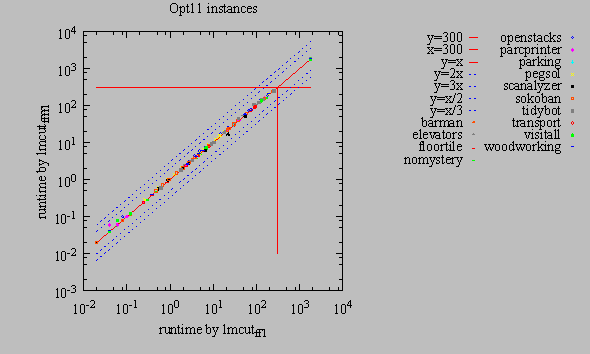
\includegraphics{tables/opt11-time-lmcut_ff-lmcut_ffff.pdf}
%  \caption{Comparison of runtime on problems solved by both single FIFO search engine (ff) and a MultiSearch engine with 2 different instances of the same FIFO engine (ffff). The runtime difference was on average below a factor of x1.1, if we ignore the subsecond differences.}
%  \label{ffff}
% \end{figure}

This portfolio strategy has several interesting theoretical characteristics. First, if we ignore the negligeble cost of insertion and deletion to the open/closed list, we do not have to pay the extra cost evaluating the heuristic function for states $f<f^*$ thanks to the caching.
Recall that \astar must always expand the states whose $f$ values are below $f^*$, the true distance from the initial state to the goal. If the heuristic estimate $h$, and in turn $f=g+h$ is the same, any tiebreaking strategy expands and evaluates the same set of nodes in $f<f*$.
Therefore, in region $f<f*$, our caching mechanism fully works and completely eliminates the possibility of extra evaluation caused by adding another queues.

Second, since the search terminates when \emph{some} engine finds a solution, and since the expansion happens in turns, the search effort within the final plateau is upper-bound by \emph{twice} the \emph{minimum} of the search efforts required by LD-LIFO or LD-FIFO engine. This is desirable because, as we saw in the last section, in some domains the gap between the best and worst tiebreaking strategy can be more than 10 times (Openstacks, for example).
When there are $n$ engines, then this increases to $n\times$ minimum
amount of effort which would be spent by each single engine.

\section{Experimental Results}

Our experimental results include 28 standard benchmark domains with
1294 problems, 16 \emph{zerocost} domains with 380 problems, 8 \emph{shuffled-zerocost} 
domains whose action ordering in the domain definition is shuffled.

We tested various tiebreaking strategies. In the following sections, we
use a convenient array-based notation of a combination of tiebreaking
strategy.  For example, $[f,h,\fd,\fifo]$ denotes standard \astar with
$h$-based first-level tiebreaking, FirstDepth second-level tiebreaking and FIFO
third-level tiebreaking.

All planners are based on the latest Fast Downward code base, and all
experiments are run using 30 minutes runtime cutoff with 2GB memory
limit. Also, experiments are conducted on Xeon E5410@2.33GHz CPUs.

\subsection{Comparison of Bucket Implementations}

We first compared well known $[f,h,\fifo]$ and $[f,h,\lifo]$, along with
$[f,h,\ro]$.
We observed that even such a slightest difference
can change the performance significantly on some domains, shown in
\reftbl{f-h-coverage}. Due to the space limitation, we show only the
domains where the difference was observed. Full table is available in
the supplemental material.

According to the result, LIFO dominates the others in Openstacks, but
Random dominates the others in Cybersec and Miconic, and FIFO dominates the others
in Airport, indicating that there are no dominance relationship between
these three and these differences are purely due to the
domain characteristics.
From this table, current benchmark set tends to be in favor of LIFO queue.

\refig{f-h-eval} gives us a more fine-grained analysis by comparing the
number of node evaluation (computations of \lmcut) on
different tiebreakings. We confirm that the difference between several
tiebreakings are sometime larger than $\times 10$.

In \reftbl{f-h-coverage}, we also added $[f,\fifo]$, $[f,\lifo]$ and
$[f,\ro]$ which does not use $h$-based first-level tiebreaking.
Interestingly, the coverage by LIFO-tiebreaking is almost comparable to
those with $h$-based tiebreaking, indicating that $h$-based tiebreaking
is not always necessary.  This is a surprising result considering
that almost all of the past literature assume the importance of the
$h$-based tiebreaking and modern forward search planners employ one.

% Note that, although LIFO dominated the others, we consider this is just by a coincidence due to our selection of problems, time limit and domains. we \emph{are not trying to claim that any of LIFO or FIFO or Random order dominates the other}. However, there are noticeable performance difference cause by these different tiebreaking strategies.

% \begin{figure}[htbp]
%  \centering \relsize{-2}
%  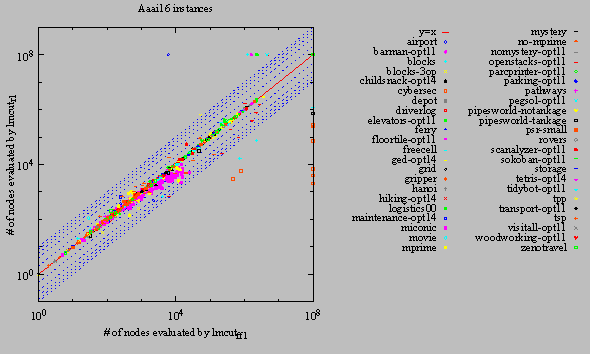
\includegraphics{tables/aaai16-evaluated-lmcut_ff-lmcut_r.pdf}
%  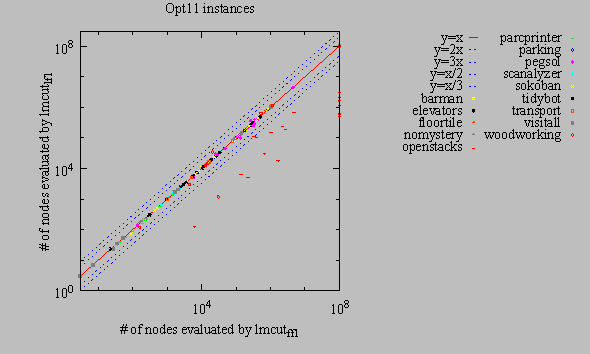
\includegraphics{tables/opt11-evaluated-lmcut_ff-lmcut_lf.pdf}
%  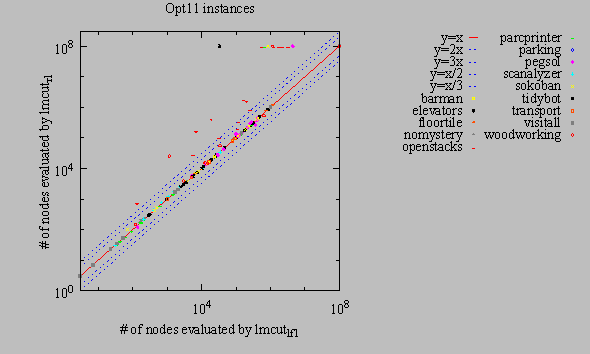
\includegraphics{tables/opt11-evaluated-lmcut_lf-lmcut_r.pdf}
%  \caption{Comparison of the number of node evaluations (computations of
%  \lmcut) by FIFO, LIFO and Random tiebreaking, on IPC2011 optimal track
%  instance. LIFO order dominates FIFO and Random order especially in
%  openstacks instances, and the gap is more than one the order of 10.}
%  \label{single-eval}
% \end{figure}
% 
\begin{table*}[htbp]
 \centering \relsize{-3}
 \begin{tabular}{|c|c|c|c|c|c|c|c|c|c|c|c|c|c||c|c|c|c|c|c|c|c|c|c|c|c||c|c||c|c|c|c|c|c|c|c|c|c|c|c||c|c|c|}
   \hline                                                                                                                           
   &  Domain & \rotatebox[origin=l]{90}{${\mbox{lmcut}}_{\mbox{ff}}$}   & \rotatebox[origin=l]{90}{${\mbox{lmcut}}_{\mbox{r}}$}   & \rotatebox[origin=l]{90}{${\mbox{lmcut}}_{\mbox{lf}}$}   & \rotatebox[origin=l]{90}{${\mbox{lmcut}}_{\mbox{${\mbox{fd}}_{\mbox{fifo}}$}}$}   & \rotatebox[origin=l]{90}{${\mbox{lmcut}}_{\mbox{${\mbox{rd}}_{\mbox{fifo}}$}}$}   & \rotatebox[origin=l]{90}{${\mbox{lmcut}}_{\mbox{${\mbox{ld}}_{\mbox{fifo}}$}}$}   & \rotatebox[origin=l]{90}{${\mbox{lmcut}}_{\mbox{${\mbox{fd}}_{\mbox{random}}$}}$}   & \rotatebox[origin=l]{90}{${\mbox{lmcut}}_{\mbox{${\mbox{rd}}_{\mbox{random}}$}}$}   & \rotatebox[origin=l]{90}{${\mbox{lmcut}}_{\mbox{${\mbox{ld}}_{\mbox{random}}$}}$}   & \rotatebox[origin=l]{90}{${\mbox{lmcut}}_{\mbox{${\mbox{fd}}_{\mbox{lifo}}$}}$}   & \rotatebox[origin=l]{90}{${\mbox{lmcut}}_{\mbox{${\mbox{rd}}_{\mbox{lifo}}$}}$}   & \rotatebox[origin=l]{90}{${\mbox{lmcut}}_{\mbox{${\mbox{ld}}_{\mbox{lifo}}$}}$}   & \rotatebox[origin=l]{90}{${\mbox{mands}}_{\mbox{ff}}$}   & \rotatebox[origin=l]{90}{${\mbox{mands}}_{\mbox{r}}$}   & \rotatebox[origin=l]{90}{${\mbox{mands}}_{\mbox{lf}}$}   & \rotatebox[origin=l]{90}{${\mbox{mands}}_{\mbox{${\mbox{fd}}_{\mbox{fifo}}$}}$}   & \rotatebox[origin=l]{90}{${\mbox{mands}}_{\mbox{${\mbox{rd}}_{\mbox{fifo}}$}}$}   & \rotatebox[origin=l]{90}{${\mbox{mands}}_{\mbox{${\mbox{ld}}_{\mbox{fifo}}$}}$}   & \rotatebox[origin=l]{90}{${\mbox{mands}}_{\mbox{${\mbox{fd}}_{\mbox{random}}$}}$}   & \rotatebox[origin=l]{90}{${\mbox{mands}}_{\mbox{${\mbox{rd}}_{\mbox{random}}$}}$}   & \rotatebox[origin=l]{90}{${\mbox{mands}}_{\mbox{${\mbox{ld}}_{\mbox{random}}$}}$}   & \rotatebox[origin=l]{90}{${\mbox{mands}}_{\mbox{${\mbox{fd}}_{\mbox{lifo}}$}}$}   & \rotatebox[origin=l]{90}{${\mbox{mands}}_{\mbox{${\mbox{rd}}_{\mbox{lifo}}$}}$}   & \rotatebox[origin=l]{90}{${\mbox{mands}}_{\mbox{${\mbox{ld}}_{\mbox{lifo}}$}}$}   & \rotatebox[origin=l]{90}{${\mbox{blind}}_{\mbox{ff}}$}   & \rotatebox[origin=l]{90}{${\mbox{blind}}_{\mbox{lf}}$}   & \rotatebox[origin=l]{90}{${\mbox{lmcut}}_{\mbox{${\mbox{ff}}_{\mbox{noh}}$}}$}   & \rotatebox[origin=l]{90}{${\mbox{lmcut}}_{\mbox{${\mbox{r}}_{\mbox{noh}}$}}$}   & \rotatebox[origin=l]{90}{${\mbox{lmcut}}_{\mbox{${\mbox{lf}}_{\mbox{noh}}$}}$}   & \rotatebox[origin=l]{90}{${\mbox{lmcut}}_{\mbox{${\mbox{fd}}_{\mbox{${\mbox{fifo}}_{\mbox{noh}}$}}$}}$}   & \rotatebox[origin=l]{90}{${\mbox{lmcut}}_{\mbox{${\mbox{rd}}_{\mbox{${\mbox{fifo}}_{\mbox{noh}}$}}$}}$}   & \rotatebox[origin=l]{90}{${\mbox{lmcut}}_{\mbox{${\mbox{ld}}_{\mbox{${\mbox{fifo}}_{\mbox{noh}}$}}$}}$}   & \rotatebox[origin=l]{90}{${\mbox{lmcut}}_{\mbox{${\mbox{fd}}_{\mbox{${\mbox{random}}_{\mbox{noh}}$}}$}}$}   & \rotatebox[origin=l]{90}{${\mbox{lmcut}}_{\mbox{${\mbox{rd}}_{\mbox{${\mbox{random}}_{\mbox{noh}}$}}$}}$}   & \rotatebox[origin=l]{90}{${\mbox{lmcut}}_{\mbox{${\mbox{ld}}_{\mbox{${\mbox{random}}_{\mbox{noh}}$}}$}}$}   & \rotatebox[origin=l]{90}{${\mbox{lmcut}}_{\mbox{${\mbox{fd}}_{\mbox{${\mbox{lifo}}_{\mbox{noh}}$}}$}}$}   & \rotatebox[origin=l]{90}{${\mbox{lmcut}}_{\mbox{${\mbox{rd}}_{\mbox{${\mbox{lifo}}_{\mbox{noh}}$}}$}}$}   & \rotatebox[origin=l]{90}{${\mbox{lmcut}}_{\mbox{${\mbox{ld}}_{\mbox{${\mbox{lifo}}_{\mbox{noh}}$}}$}}$}   & \rotatebox[origin=l]{90}{${\mbox{mands}}_{\mbox{${\mbox{ff}}_{\mbox{noh}}$}}$}   & \rotatebox[origin=l]{90}{${\mbox{mands}}_{\mbox{${\mbox{r}}_{\mbox{noh}}$}}$}   & \rotatebox[origin=l]{90}{${\mbox{mands}}_{\mbox{${\mbox{lf}}_{\mbox{noh}}$}}$}    \\
   \hline                                                                                                                           
   &  Sum &  560 &  556 &  \textbf{565} &  0 &  0 &  0 &  0 &  0 &  0 &  0 &  0 &  0 &  489 &  470 &  \textbf{496} &  0 &  0 &  0 &  0 &  0 &  0 &  0 &  0 &  0 &  402 &  \textbf{408} &  445 &  445 &  \textbf{559} &  0 &  0 &  0 &  0 &  0 &  0 &  0 &  0 &  0 &  460 &  422 &  \textbf{491}  \\
   \hline                                                                                                                           
\multirow{35}{*}{\rotatebox[origin=c]{90}{\textbf{LMcut Benchmark Suite+}}}   &  {\relsize{-1}airport(50)} &  \textbf{27} &  25 &  26 &  0 &  0 &  0 &  0 &  0 &  0 &  0 &  0 &  0 &  \textbf{9} &  \textbf{9} &  \textbf{9} &  0 &  0 &  0 &  0 &  0 &  0 &  0 &  0 &  0 &  18 &  18 &  18 &  18 &  \textbf{26} &  0 &  0 &  0 &  0 &  0 &  0 &  0 &  0 &  0 &  9 &  9 &  9  \\
   &  {\relsize{-1}barman-opt11(20)} &  0 &  0 &  0 &  0 &  0 &  0 &  0 &  0 &  0 &  0 &  0 &  0 &  \textbf{4} &  \textbf{4} &  \textbf{4} &  0 &  0 &  0 &  0 &  0 &  0 &  0 &  0 &  0 &  4 &  4 &  0 &  0 &  0 &  0 &  0 &  0 &  0 &  0 &  0 &  0 &  0 &  0 &  4 &  4 &  4  \\
   &  {\relsize{-1}blocks(35)} &  \textbf{28} &  \textbf{28} &  \textbf{28} &  0 &  0 &  0 &  0 &  0 &  0 &  0 &  0 &  0 &  \textbf{22} &  \textbf{22} &  \textbf{22} &  0 &  0 &  0 &  0 &  0 &  0 &  0 &  0 &  0 &  18 &  18 &  26 &  26 &  \textbf{27} &  0 &  0 &  0 &  0 &  0 &  0 &  0 &  0 &  0 &  21 &  19 &  \textbf{22}  \\
   &  {\relsize{-1}cybersec(19)} &  1 &  \textbf{2} &  \textbf{2} &  0 &  0 &  0 &  0 &  0 &  0 &  0 &  0 &  0 &  0 &  0 &  0 &  0 &  0 &  0 &  0 &  0 &  0 &  0 &  0 &  0 &  0 &  0 &  0 &  0 &  \textbf{1} &  0 &  0 &  0 &  0 &  0 &  0 &  0 &  0 &  0 &  0 &  0 &  0  \\
   &  {\relsize{-1}depot(22)} &  \textbf{6} &  \textbf{6} &  \textbf{6} &  0 &  0 &  0 &  0 &  0 &  0 &  0 &  0 &  0 &  \textbf{6} &  5 &  \textbf{6} &  0 &  0 &  0 &  0 &  0 &  0 &  0 &  0 &  0 &  4 &  4 &  5 &  5 &  \textbf{6} &  0 &  0 &  0 &  0 &  0 &  0 &  0 &  0 &  0 &  5 &  4 &  \textbf{6}  \\
   &  {\relsize{-1}driverlog(20)} &  \textbf{13} &  \textbf{13} &  \textbf{13} &  0 &  0 &  0 &  0 &  0 &  0 &  0 &  0 &  0 &  \textbf{12} &  \textbf{12} &  \textbf{12} &  0 &  0 &  0 &  0 &  0 &  0 &  0 &  0 &  0 &  7 &  7 &  12 &  12 &  \textbf{13} &  0 &  0 &  0 &  0 &  0 &  0 &  0 &  0 &  0 &  \textbf{12} &  11 &  \textbf{12}  \\
   &  {\relsize{-1}elevators-opt11(20)} &  \textbf{15} &  \textbf{15} &  \textbf{15} &  0 &  0 &  0 &  0 &  0 &  0 &  0 &  0 &  0 &  \textbf{13} &  12 &  \textbf{13} &  0 &  0 &  0 &  0 &  0 &  0 &  0 &  0 &  0 &  9 &  9 &  14 &  14 &  \textbf{15} &  0 &  0 &  0 &  0 &  0 &  0 &  0 &  0 &  0 &  \textbf{13} &  10 &  \textbf{13}  \\
   &  {\relsize{-1}floortile-opt11(20)} &  \textbf{6} &  \textbf{6} &  \textbf{6} &  0 &  0 &  0 &  0 &  0 &  0 &  0 &  0 &  0 &  \textbf{6} &  \textbf{6} &  \textbf{6} &  0 &  0 &  0 &  0 &  0 &  0 &  0 &  0 &  0 &  2 &  2 &  \textbf{6} &  \textbf{6} &  \textbf{6} &  0 &  0 &  0 &  0 &  0 &  0 &  0 &  0 &  0 &  5 &  4 &  \textbf{6}  \\
   &  {\relsize{-1}freecell(80)} &  \textbf{9} &  \textbf{9} &  \textbf{9} &  0 &  0 &  0 &  0 &  0 &  0 &  0 &  0 &  0 &  \textbf{17} &  15 &  \textbf{17} &  0 &  0 &  0 &  0 &  0 &  0 &  0 &  0 &  0 &  15 &  15 &  8 &  \textbf{9} &  \textbf{9} &  0 &  0 &  0 &  0 &  0 &  0 &  0 &  0 &  0 &  15 &  14 &  \textbf{16}  \\
   &  {\relsize{-1}grid(5)} &  \textbf{1} &  \textbf{1} &  \textbf{1} &  0 &  0 &  0 &  0 &  0 &  0 &  0 &  0 &  0 &  \textbf{2} &  \textbf{2} &  \textbf{2} &  0 &  0 &  0 &  0 &  0 &  0 &  0 &  0 &  0 &  1 &  1 &  \textbf{1} &  \textbf{1} &  \textbf{1} &  0 &  0 &  0 &  0 &  0 &  0 &  0 &  0 &  0 &  2 &  2 &  2  \\
   &  {\relsize{-1}gripper(20)} &  \textbf{6} &  \textbf{6} &  \textbf{6} &  0 &  0 &  0 &  0 &  0 &  0 &  0 &  0 &  0 &  \textbf{20} &  \textbf{20} &  \textbf{20} &  0 &  0 &  0 &  0 &  0 &  0 &  0 &  0 &  0 &  7 &  7 &  \textbf{6} &  \textbf{6} &  \textbf{6} &  0 &  0 &  0 &  0 &  0 &  0 &  0 &  0 &  0 &  8 &  6 &  \textbf{20}  \\
   &  {\relsize{-1}hanoi(30)} &  \textbf{12} &  \textbf{12} &  \textbf{12} &  0 &  0 &  0 &  0 &  0 &  0 &  0 &  0 &  0 &  \textbf{14} &  \textbf{14} &  \textbf{14} &  0 &  0 &  0 &  0 &  0 &  0 &  0 &  0 &  0 &  12 &  12 &  \textbf{12} &  \textbf{12} &  \textbf{12} &  0 &  0 &  0 &  0 &  0 &  0 &  0 &  0 &  0 &  14 &  14 &  14  \\
   &  {\relsize{-1}logistics00(28)} &  \textbf{20} &  \textbf{20} &  \textbf{20} &  0 &  0 &  0 &  0 &  0 &  0 &  0 &  0 &  0 &  \textbf{20} &  \textbf{20} &  \textbf{20} &  0 &  0 &  0 &  0 &  0 &  0 &  0 &  0 &  0 &  10 &  10 &  16 &  16 &  \textbf{19} &  0 &  0 &  0 &  0 &  0 &  0 &  0 &  0 &  0 &  \textbf{20} &  17 &  \textbf{20}  \\
   &  {\relsize{-1}miconic(150)} &  \textbf{140} &  \textbf{140} &  \textbf{140} &  0 &  0 &  0 &  0 &  0 &  0 &  0 &  0 &  0 &  \textbf{73} &  72 &  \textbf{73} &  0 &  0 &  0 &  0 &  0 &  0 &  0 &  0 &  0 &  49 &  \textbf{50} &  68 &  68 &  \textbf{140} &  0 &  0 &  0 &  0 &  0 &  0 &  0 &  0 &  0 &  68 &  68 &  \textbf{73}  \\
   &  {\relsize{-1}mprime(35)} &  \textbf{21} &  \textbf{21} &  \textbf{21} &  0 &  0 &  0 &  0 &  0 &  0 &  0 &  0 &  0 &  23 &  23 &  \textbf{24} &  0 &  0 &  0 &  0 &  0 &  0 &  0 &  0 &  0 &  19 &  19 &  20 &  19 &  \textbf{22} &  0 &  0 &  0 &  0 &  0 &  0 &  0 &  0 &  0 &  \textbf{23} &  22 &  \textbf{23}  \\
   &  {\relsize{-1}mystery(30)} &  \textbf{16} &  15 &  \textbf{16} &  0 &  0 &  0 &  0 &  0 &  0 &  0 &  0 &  0 &  15 &  15 &  \textbf{16} &  0 &  0 &  0 &  0 &  0 &  0 &  0 &  0 &  0 &  15 &  15 &  15 &  15 &  \textbf{16} &  0 &  0 &  0 &  0 &  0 &  0 &  0 &  0 &  0 &  15 &  15 &  15  \\
   &  {\relsize{-1}nomystery-opt11(20)} &  \textbf{14} &  \textbf{14} &  \textbf{14} &  0 &  0 &  0 &  0 &  0 &  0 &  0 &  0 &  0 &  \textbf{18} &  \textbf{18} &  \textbf{18} &  0 &  0 &  0 &  0 &  0 &  0 &  0 &  0 &  0 &  8 &  8 &  12 &  12 &  \textbf{13} &  0 &  0 &  0 &  0 &  0 &  0 &  0 &  0 &  0 &  17 &  16 &  \textbf{18}  \\
   &  {\relsize{-1}openstacks-opt11(20)} &  12 &  10 &  \textbf{18} &  0 &  0 &  0 &  0 &  0 &  0 &  0 &  0 &  0 &  15 &  10 &  \textbf{19} &  0 &  0 &  0 &  0 &  0 &  0 &  0 &  0 &  0 &  15 &  \textbf{19} &  12 &  10 &  \textbf{18} &  0 &  0 &  0 &  0 &  0 &  0 &  0 &  0 &  0 &  15 &  9 &  \textbf{19}  \\
   &  {\relsize{-1}parcprinter-opt11(20)} &  \textbf{13} &  \textbf{13} &  \textbf{13} &  0 &  0 &  0 &  0 &  0 &  0 &  0 &  0 &  0 &  \textbf{10} &  \textbf{10} &  \textbf{10} &  0 &  0 &  0 &  0 &  0 &  0 &  0 &  0 &  0 &  6 &  6 &  12 &  12 &  \textbf{13} &  0 &  0 &  0 &  0 &  0 &  0 &  0 &  0 &  0 &  10 &  10 &  10  \\
   &  {\relsize{-1}parking-opt11(20)} &  \textbf{1} &  \textbf{1} &  \textbf{1} &  0 &  0 &  0 &  0 &  0 &  0 &  0 &  0 &  0 &  \textbf{1} &  \textbf{1} &  \textbf{1} &  0 &  0 &  0 &  0 &  0 &  0 &  0 &  0 &  0 &  0 &  0 &  \textbf{1} &  \textbf{1} &  \textbf{1} &  0 &  0 &  0 &  0 &  0 &  0 &  0 &  0 &  0 &  1 &  1 &  1  \\
   &  {\relsize{-1}pathways(30)} &  \textbf{5} &  \textbf{5} &  \textbf{5} &  0 &  0 &  0 &  0 &  0 &  0 &  0 &  0 &  0 &  \textbf{4} &  \textbf{4} &  \textbf{4} &  0 &  0 &  0 &  0 &  0 &  0 &  0 &  0 &  0 &  4 &  4 &  4 &  4 &  \textbf{5} &  0 &  0 &  0 &  0 &  0 &  0 &  0 &  0 &  0 &  4 &  4 &  4  \\
   &  {\relsize{-1}pegsol-opt11(20)} &  \textbf{17} &  \textbf{17} &  \textbf{17} &  0 &  0 &  0 &  0 &  0 &  0 &  0 &  0 &  0 &  \textbf{19} &  18 &  \textbf{19} &  0 &  0 &  0 &  0 &  0 &  0 &  0 &  0 &  0 &  17 &  17 &  \textbf{17} &  16 &  \textbf{17} &  0 &  0 &  0 &  0 &  0 &  0 &  0 &  0 &  0 &  17 &  16 &  \textbf{19}  \\
   &  {\relsize{-1}pipesworld-notankage(50)} &  \textbf{15} &  \textbf{15} &  \textbf{15} &  0 &  0 &  0 &  0 &  0 &  0 &  0 &  0 &  0 &  8 &  8 &  \textbf{9} &  0 &  0 &  0 &  0 &  0 &  0 &  0 &  0 &  0 &  14 &  14 &  \textbf{13} &  \textbf{13} &  \textbf{13} &  0 &  0 &  0 &  0 &  0 &  0 &  0 &  0 &  0 &  8 &  8 &  \textbf{10}  \\
   &  {\relsize{-1}pipesworld-tankage(50)} &  \textbf{8} &  \textbf{8} &  \textbf{8} &  0 &  0 &  0 &  0 &  0 &  0 &  0 &  0 &  0 &  \textbf{13} &  12 &  \textbf{13} &  0 &  0 &  0 &  0 &  0 &  0 &  0 &  0 &  0 &  10 &  \textbf{11} &  7 &  \textbf{8} &  \textbf{8} &  0 &  0 &  0 &  0 &  0 &  0 &  0 &  0 &  0 &  \textbf{13} &  12 &  \textbf{13}  \\
   &  {\relsize{-1}psr-small(50)} &  \textbf{48} &  \textbf{48} &  \textbf{48} &  0 &  0 &  0 &  0 &  0 &  0 &  0 &  0 &  0 &  \textbf{50} &  \textbf{50} &  \textbf{50} &  0 &  0 &  0 &  0 &  0 &  0 &  0 &  0 &  0 &  49 &  49 &  \textbf{48} &  \textbf{48} &  \textbf{48} &  0 &  0 &  0 &  0 &  0 &  0 &  0 &  0 &  0 &  \textbf{50} &  48 &  \textbf{50}  \\
   &  {\relsize{-1}rovers(40)} &  \textbf{7} &  \textbf{7} &  \textbf{7} &  0 &  0 &  0 &  0 &  0 &  0 &  0 &  0 &  0 &  \textbf{8} &  6 &  \textbf{8} &  0 &  0 &  0 &  0 &  0 &  0 &  0 &  0 &  0 &  5 &  5 &  \textbf{7} &  \textbf{7} &  \textbf{7} &  0 &  0 &  0 &  0 &  0 &  0 &  0 &  0 &  0 &  7 &  5 &  \textbf{8}  \\
   &  {\relsize{-1}scanalyzer-opt11(20)} &  \textbf{10} &  \textbf{10} &  \textbf{10} &  0 &  0 &  0 &  0 &  0 &  0 &  0 &  0 &  0 &  \textbf{10} &  9 &  \textbf{10} &  0 &  0 &  0 &  0 &  0 &  0 &  0 &  0 &  0 &  9 &  9 &  4 &  4 &  \textbf{10} &  0 &  0 &  0 &  0 &  0 &  0 &  0 &  0 &  0 &  \textbf{10} &  7 &  \textbf{10}  \\
   &  {\relsize{-1}sokoban-opt11(20)} &  \textbf{19} &  \textbf{19} &  \textbf{19} &  0 &  0 &  0 &  0 &  0 &  0 &  0 &  0 &  0 &  \textbf{20} &  19 &  \textbf{20} &  0 &  0 &  0 &  0 &  0 &  0 &  0 &  0 &  0 &  18 &  18 &  \textbf{19} &  \textbf{19} &  \textbf{19} &  0 &  0 &  0 &  0 &  0 &  0 &  0 &  0 &  0 &  \textbf{20} &  16 &  \textbf{20}  \\
   &  {\relsize{-1}storage(30)} &  \textbf{15} &  \textbf{15} &  14 &  0 &  0 &  0 &  0 &  0 &  0 &  0 &  0 &  0 &  \textbf{15} &  \textbf{15} &  \textbf{15} &  0 &  0 &  0 &  0 &  0 &  0 &  0 &  0 &  0 &  14 &  14 &  \textbf{14} &  \textbf{14} &  \textbf{14} &  0 &  0 &  0 &  0 &  0 &  0 &  0 &  0 &  0 &  \textbf{15} &  14 &  \textbf{15}  \\
   &  {\relsize{-1}tidybot-opt11(20)} &  \textbf{12} &  \textbf{12} &  \textbf{12} &  0 &  0 &  0 &  0 &  0 &  0 &  0 &  0 &  0 &  0 &  0 &  0 &  0 &  0 &  0 &  0 &  0 &  0 &  0 &  0 &  0 &  12 &  12 &  11 &  11 &  \textbf{12} &  0 &  0 &  0 &  0 &  0 &  0 &  0 &  0 &  0 &  0 &  0 &  0  \\
   &  {\relsize{-1}tpp(30)} &  \textbf{6} &  \textbf{6} &  \textbf{6} &  0 &  0 &  0 &  0 &  0 &  0 &  0 &  0 &  0 &  \textbf{7} &  6 &  \textbf{7} &  0 &  0 &  0 &  0 &  0 &  0 &  0 &  0 &  0 &  6 &  6 &  \textbf{6} &  \textbf{6} &  \textbf{6} &  0 &  0 &  0 &  0 &  0 &  0 &  0 &  0 &  0 &  6 &  6 &  6  \\
   &  {\relsize{-1}transport-opt11(20)} &  \textbf{6} &  \textbf{6} &  \textbf{6} &  0 &  0 &  0 &  0 &  0 &  0 &  0 &  0 &  0 &  \textbf{7} &  \textbf{7} &  \textbf{7} &  0 &  0 &  0 &  0 &  0 &  0 &  0 &  0 &  0 &  6 &  6 &  \textbf{6} &  \textbf{6} &  \textbf{6} &  0 &  0 &  0 &  0 &  0 &  0 &  0 &  0 &  0 &  \textbf{7} &  6 &  \textbf{7}  \\
   &  {\relsize{-1}visitall-opt11(20)} &  \textbf{10} &  \textbf{10} &  \textbf{10} &  0 &  0 &  0 &  0 &  0 &  0 &  0 &  0 &  0 &  \textbf{9} &  \textbf{9} &  \textbf{9} &  0 &  0 &  0 &  0 &  0 &  0 &  0 &  0 &  0 &  9 &  9 &  \textbf{10} &  \textbf{10} &  \textbf{10} &  0 &  0 &  0 &  0 &  0 &  0 &  0 &  0 &  0 &  9 &  9 &  9  \\
   &  {\relsize{-1}woodworking-opt11(20)} &  \textbf{10} &  \textbf{10} &  \textbf{10} &  0 &  0 &  0 &  0 &  0 &  0 &  0 &  0 &  0 &  \textbf{7} &  \textbf{7} &  \textbf{7} &  0 &  0 &  0 &  0 &  0 &  0 &  0 &  0 &  0 &  2 &  2 &  6 &  8 &  \textbf{9} &  0 &  0 &  0 &  0 &  0 &  0 &  0 &  0 &  0 &  7 &  7 &  7  \\
   &  {\relsize{-1}zenotravel(20)} &  \textbf{11} &  \textbf{11} &  \textbf{11} &  0 &  0 &  0 &  0 &  0 &  0 &  0 &  0 &  0 &  \textbf{12} &  10 &  \textbf{12} &  0 &  0 &  0 &  0 &  0 &  0 &  0 &  0 &  0 &  8 &  8 &  9 &  9 &  \textbf{11} &  0 &  0 &  0 &  0 &  0 &  0 &  0 &  0 &  0 &  \textbf{10} &  9 &  \textbf{10} \\
\hline
   &  Sum &  163 &  163 &  166 &  163 &  175 &  \textbf{177} &  158 &  172 &  173 &  164 &  167 &  165 &  170 &  165 &  170 &  169 &  \textbf{176} &  \textbf{176} &  161 &  173 &  171 &  168 &  167 &  165 &  116 &  \textbf{117} &  137 &  130 &  167 &  137 &  165 &  \textbf{172} &  133 &  169 &  170 &  139 &  164 &  166 &  148 &  134 &  \textbf{169}  \\
   \hline                                                                                                                           
\multirow{16}{*}{\rotatebox[origin=c]{90}{}}   &  {\relsize{-1}airport-fuel(20)} &  \textbf{15} &  14 &  14 &  \textbf{15} &  14 &  14 &  14 &  13 &  13 &  14 &  \textbf{15} &  14 &  5 &  5 &  5 &  5 &  5 &  5 &  5 &  5 &  5 &  5 &  5 &  5 &  7 &  7 &  7 &  7 &  \textbf{15} &  7 &  10 &  14 &  8 &  10 &  14 &  8 &  12 &  \textbf{15} &  5 &  5 &  5  \\
   &  {\relsize{-1}depot-fuel(22)} &  6 &  6 &  6 &  6 &  6 &  6 &  6 &  6 &  6 &  6 &  6 &  6 &  5 &  3 &  5 &  5 &  5 &  4 &  3 &  \textbf{6} &  4 &  5 &  5 &  3 &  5 &  5 &  5 &  5 &  \textbf{6} &  5 &  \textbf{6} &  \textbf{6} &  5 &  \textbf{6} &  \textbf{6} &  5 &  \textbf{6} &  \textbf{6} &  \textbf{5} &  3 &  \textbf{5}  \\
   &  {\relsize{-1}driverlog-fuel(20)} &  \textbf{8} &  \textbf{8} &  \textbf{8} &  \textbf{8} &  \textbf{8} &  7 &  \textbf{8} &  \textbf{8} &  7 &  \textbf{8} &  \textbf{8} &  7 &  \textbf{9} &  8 &  \textbf{9} &  \textbf{9} &  \textbf{9} &  8 &  8 &  \textbf{9} &  8 &  \textbf{9} &  \textbf{9} &  8 &  \textbf{6} &  5 &  7 &  5 &  \textbf{8} &  7 &  \textbf{8} &  6 &  6 &  \textbf{8} &  5 &  7 &  7 &  7 &  8 &  8 &  \textbf{9}  \\
   &  {\relsize{-1}floortile-ink(20)} &  8 &  8 &  8 &  8 &  8 &  8 &  8 &  8 &  8 &  8 &  8 &  8 &  \textbf{8} &  \textbf{8} &  \textbf{8} &  7 &  7 &  7 &  6 &  7 &  7 &  6 &  7 &  6 &  2 &  2 &  8 &  8 &  8 &  8 &  8 &  8 &  8 &  8 &  8 &  8 &  8 &  8 &  \textbf{8} &  4 &  \textbf{8}  \\
   &  {\relsize{-1}ged-opt14(20)} &  15 &  15 &  15 &  15 &  15 &  15 &  15 &  15 &  15 &  15 &  15 &  15 &  15 &  15 &  15 &  15 &  15 &  15 &  15 &  15 &  15 &  15 &  15 &  15 &  15 &  15 &  \textbf{15} &  14 &  \textbf{15} &  \textbf{15} &  13 &  13 &  13 &  \textbf{15} &  14 &  \textbf{15} &  \textbf{15} &  \textbf{15} &  \textbf{15} &  14 &  \textbf{15}  \\
   &  {\relsize{-1}grid-fuel(5)} &  1 &  1 &  1 &  1 &  1 &  1 &  1 &  1 &  1 &  1 &  1 &  1 &  2 &  2 &  2 &  2 &  2 &  2 &  2 &  2 &  2 &  2 &  2 &  2 &  1 &  1 &  1 &  1 &  1 &  1 &  1 &  1 &  1 &  1 &  1 &  1 &  1 &  1 &  2 &  2 &  2  \\
   &  {\relsize{-1}hiking-fuel(20)} &  9 &  9 &  9 &  9 &  9 &  9 &  9 &  9 &  9 &  9 &  9 &  9 &  \textbf{13} &  11 &  \textbf{13} &  \textbf{13} &  \textbf{13} &  \textbf{13} &  11 &  11 &  11 &  \textbf{13} &  \textbf{13} &  \textbf{13} &  11 &  11 &  8 &  8 &  \textbf{9} &  8 &  \textbf{9} &  \textbf{9} &  8 &  \textbf{9} &  \textbf{9} &  8 &  \textbf{9} &  \textbf{9} &  \textbf{13} &  11 &  \textbf{13}  \\
   &  {\relsize{-1}logistics00-fuel(28)} &  \textbf{16} &  15 &  \textbf{16} &  \textbf{16} &  \textbf{16} &  \textbf{16} &  15 &  15 &  15 &  \textbf{16} &  \textbf{16} &  \textbf{16} &  16 &  16 &  16 &  16 &  16 &  16 &  16 &  16 &  16 &  16 &  16 &  16 &  10 &  10 &  15 &  15 &  \textbf{16} &  15 &  \textbf{16} &  15 &  15 &  15 &  15 &  15 &  \textbf{16} &  \textbf{16} &  16 &  16 &  16  \\
   &  {\relsize{-1}miconic-up(30)} &  16 &  17 &  18 &  16 &  \textbf{20} &  \textbf{20} &  15 &  \textbf{20} &  \textbf{20} &  16 &  18 &  18 &  29 &  \textbf{30} &  \textbf{30} &  29 &  \textbf{30} &  \textbf{30} &  29 &  \textbf{30} &  \textbf{30} &  29 &  \textbf{30} &  \textbf{30} &  \textbf{9} &  8 &  10 &  10 &  18 &  10 &  \textbf{20} &  \textbf{20} &  10 &  19 &  18 &  10 &  19 &  18 &  19 &  20 &  \textbf{30}  \\
   &  {\relsize{-1}mprime-succumb(35)} &  15 &  16 &  14 &  15 &  21 &  \textbf{25} &  15 &  21 &  23 &  17 &  15 &  14 &  21 &  20 &  19 &  21 &  25 &  \textbf{27} &  19 &  23 &  24 &  21 &  17 &  19 &  \textbf{4} &  3 &  12 &  9 &  14 &  12 &  21 &  \textbf{25} &  11 &  20 &  23 &  13 &  14 &  14 &  14 &  10 &  \textbf{19}  \\
   &  {\relsize{-1}nomystery-fuel(20)} &  10 &  10 &  10 &  10 &  10 &  10 &  10 &  10 &  10 &  10 &  10 &  10 &  16 &  16 &  16 &  16 &  16 &  16 &  16 &  16 &  16 &  16 &  16 &  16 &  8 &  8 &  9 &  9 &  \textbf{10} &  9 &  9 &  9 &  9 &  \textbf{10} &  \textbf{10} &  9 &  \textbf{10} &  \textbf{10} &  15 &  15 &  \textbf{16}  \\
   &  {\relsize{-1}pathways-fuel(30)} &  \textbf{5} &  \textbf{5} &  \textbf{5} &  \textbf{5} &  \textbf{5} &  4 &  4 &  4 &  4 &  \textbf{5} &  \textbf{5} &  \textbf{5} &  4 &  4 &  4 &  4 &  4 &  4 &  4 &  4 &  4 &  4 &  4 &  4 &  4 &  4 &  4 &  4 &  \textbf{5} &  4 &  4 &  4 &  4 &  \textbf{5} &  4 &  4 &  \textbf{5} &  \textbf{5} &  4 &  4 &  4  \\
   &  {\relsize{-1}rovers-fuel(40)} &  8 &  8 &  8 &  8 &  8 &  8 &  8 &  8 &  8 &  8 &  8 &  8 &  8 &  8 &  8 &  8 &  8 &  8 &  8 &  8 &  8 &  8 &  8 &  8 &  6 &  6 &  7 &  7 &  \textbf{9} &  7 &  8 &  \textbf{9} &  7 &  \textbf{9} &  \textbf{9} &  7 &  \textbf{9} &  \textbf{9} &  8 &  8 &  8  \\
   &  {\relsize{-1}tidybot-motion(20)} &  16 &  16 &  16 &  16 &  16 &  16 &  16 &  16 &  16 &  16 &  16 &  16 &  0 &  0 &  0 &  0 &  0 &  0 &  0 &  0 &  0 &  0 &  0 &  0 &  15 &  \textbf{17} &  14 &  14 &  15 &  14 &  15 &  15 &  14 &  \textbf{16} &  \textbf{16} &  14 &  \textbf{16} &  15 &  0 &  0 &  0  \\
   &  {\relsize{-1}tpp-fuel(30)} &  8 &  8 &  \textbf{11} &  8 &  \textbf{11} &  \textbf{11} &  7 &  \textbf{11} &  \textbf{11} &  8 &  10 &  \textbf{11} &  9 &  9 &  10 &  9 &  \textbf{11} &  \textbf{11} &  9 &  \textbf{11} &  \textbf{11} &  9 &  10 &  10 &  6 &  \textbf{8} &  8 &  7 &  \textbf{11} &  8 &  10 &  \textbf{11} &  7 &  \textbf{11} &  \textbf{11} &  8 &  10 &  \textbf{11} &  8 &  7 &  \textbf{10}  \\
   &  {\relsize{-1}zenotravel-fuel(20)} &  7 &  7 &  7 &  7 &  7 &  7 &  7 &  7 &  7 &  7 &  7 &  7 &  10 &  10 &  10 &  10 &  10 &  10 &  10 &  10 &  10 &  10 &  10 &  10 &  7 &  7 &  7 &  7 &  7 &  7 &  7 &  7 &  7 &  7 &  7 &  7 &  7 &  7 &  8 &  7 &  \textbf{9} \\
\hline
   &  Total &  723 &  719 &  \textbf{731} &  163 &  175 &  177 &  158 &  172 &  173 &  164 &  167 &  165 &  659 &  635 &  \textbf{666} &  169 &  176 &  176 &  161 &  173 &  171 &  168 &  167 &  165 &  518 &  \textbf{525} &  582 &  575 &  \textbf{726} &  137 &  165 &  172 &  133 &  169 &  170 &  139 &  164 &  166 &  608 &  556 &  \textbf{660} \\
\hline
\end{tabular}

 \caption{Preliminary experiments comparing the performance of FIFO,
 LIFO and Random second-level tiebreaking using Fast Downward. Each cell
 denotes the problem solved with 30 minutes runtime, 2GB memory
 limitation. \textbf{Boldface} denotes the case where it achieved the
 best result among configurations.} \label{single-coverage}
\end{table*}

\subsection{Size of the Plateau Matters}

We also observed that, such differences occur especially in the problems which
have the huge search plateau, i.e., the problems where the heuristic
function is not informative and the planner relies heavily on the
tiebreaking criteria.
% 
\refig{plateau-f-h} plots in $y$-axis the initial size of the tiebreaking bucket in
which the goal node was found, compared to the total number of
evaluation in $x$-axis. Tiebreaking bucket is a set of open nodes in which the
nodes share the same sort key $[f,h]$, or $[f]$ when $h$-tiebraking is
disabled. 
The figure shows the result from $[f,h,\fifo]$ tiebreaking, however in
theory the initial size of the bucket does not change among
$[f,h,\fifo]$, $[f,h,\lifo]$ and $[f,h,\ro]$ as long as the size
is measured when it is encountered for the first time.

Although the initial number of nodes in the plateau is only a lower
bound of entire nodes in the plateau (including unexpanded ones), from
this figure the planner cound spend almost tenth of the runtime on
searching through the final plateau in the worst case. This means that
these domains have very large variance in the runtime caused by the
difference in second-level tiebreakings.

%  For example, FIFO, LIFO and RO would respectively
% perform better if the goal nodes exist near the beginning of the bucket,
% near the end of the bucket, or
% % is evenly distributed among the bucket.
% is densely populated in a narrow region somewhere in the midst of the bucket when the
% search proceeds to the new $[f,h]$ plateau.
% 
\refig{plateau-h} is a similar plot where the $h$-based tiebreaking is
disabled. As expected, much larger effort is spent on the final plateau
without $h$-based tiebreaking.

\begin{figure}[htb]
 \centering
 \relsize{-3}
 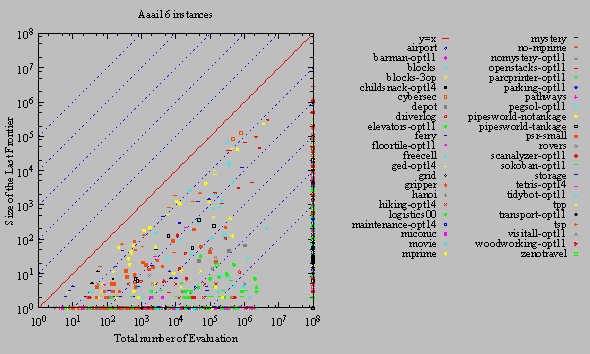
\includegraphics{tables/aaai16-front-vs-evaluated.pdf}
 \caption{Comparison of the size of the search plateau compared to the total evaluation. Data were obtained by the result of standard FIFO tiebreaking on the standard benchmark instances. Both axes are logarithmic. Each dotted line represents 10x, 100x ... lines.  Openstacks,  clearly has the large plateaus.}
 \label{plateau-h}
\end{figure}

\begin{figure}[htb]
 \centering
 \relsize{-2}
 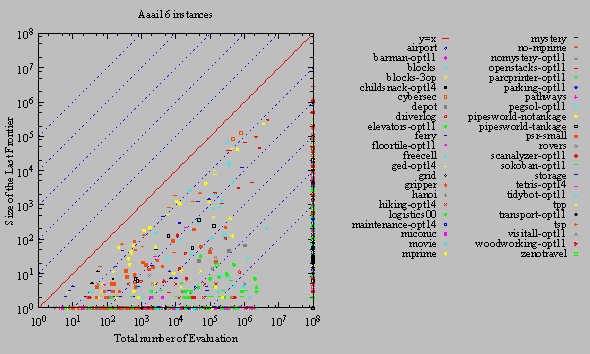
\includegraphics{tables/aaai16-front-vs-evaluated.pdf}
 \caption{Comparison of the size of the search plateau compared to the total evaluation. Data were obtained by the result of running \astar on the standard benchmark instances, with FIFO but without the tiebreaking by $h$. Both axes are logarithmic. Each dotted line represents 10x, 100x ... lines.}
 \label{plateau-f}
\end{figure}

% We can have several important observations from these results.  Firstly, in a plateau, \textbf{the heuristic functions are not used at all, nor the search is guided at all}. This observation holds even if we combine several nondominating heuristics e.g. \lmcut and M\&S, regardress of the method, e.g., taking the maximum, using portfolio or utilize them as the first tiebreaking strategy. It is still possible that a plateau is encountered, since it is not a perfect heuristics yet!
% Such a plateau is known to be inevitable even if we have an almost perfect heuristics $h_c$, and it is impossible to improve upon $h_c$ --- if it could, the result would be a perfect heuristics or an inadmissible heuristics. Therefore, this problem cannot be solved by improving the heuristic accuracy, which is the currently dominating meta-strategy to improve the planner performance.
% 
% Secondly, there is no legitimate reason which supports each tiebreaking strategy.
% As long as $f$-value is the first sort key, any tiebreaking criteria are admissible. \textbf{$h$ and FIFO are just heuristically chosen by the implementer of the planner.} Nor are there any reason to choose LIFO or Random tie breaking. Moreover, the different seed value of a Random tiebreaking yield the different search behavior and different result. (In all of our experiment we fixed the seed to 1.)

% Based on these observation, the next step we have taken is to develop a new
% portfolio-based multi-tiebreaking strategy \textbf{which is orthogonal to
% the approach of improving the heuristic accuracy.}

% The following sections are devoted to giving further analysis on the
% reason behind their behavior.

\subsection{Evaluating Depth-based Tiebreaking}




\subsection{Evaluating MultiSearch Strategy}

Finally, we conducted experiments for evaluating our MultiSearch strategy.
% the number of evaluations and expansions, along with 
\refig{portfolio-ff} to \refig{portfolio-r} shows the runtime between different combinations of 2 or 3 tiebreaking strategies (FIFO+LIFO, FIFO+Random, LIFO+Random, FIFO+LIFO+Random) and the single tiebreaking strategies. The results support our claim that the evaluation never exceeds twice/thirds of the single search engine and, in practice, the evaluations are mostly the same with the single search engine, and in some domains with large plateaus, the search effort used by MultiSearch is more than ten times less than by the single strategy.

\begin{figure}[htbp]
 \centering
 \relsize{-2}
 % 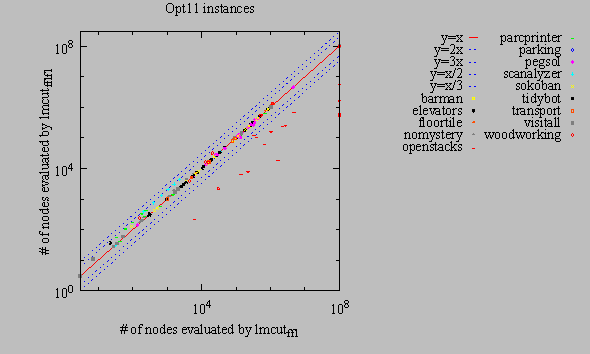
\includegraphics{tables/opt11-evaluated-lmcut_ff-lmcut_fflf.pdf}
 % 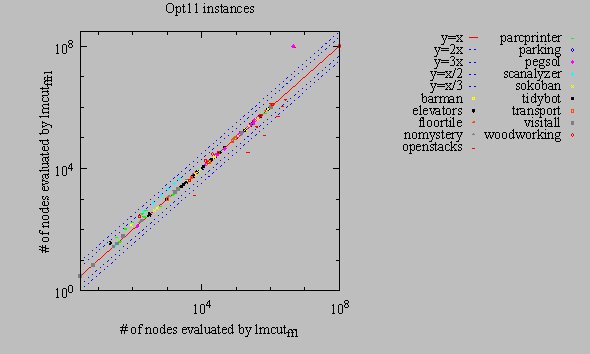
\includegraphics{tables/opt11-evaluated-lmcut_ff-lmcut_ffr.pdf}
 % 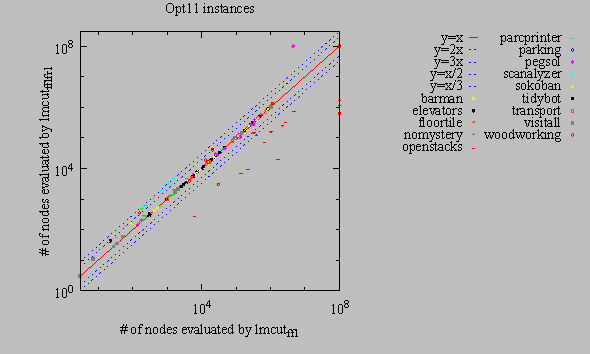
\includegraphics{tables/opt11-evaluated-lmcut_ff-lmcut_fflfr.pdf}
 \caption{}
 \label{portfolio-ff}
\end{figure}


\section{Related Work}
\label{sec-4}

\emph{Symmetry Breaking} \cite{Fox1998,pochter2011exploiting,domshlak2013symmetry} is the search technique that tries to prune the states with symmetric paths. \emph{Partial Order Reduction}, \emph{Strong Stubbern Sets} and \emph{Expansion Core} are also the techniques which prune the intermediate states that reach to the same goal using the different orders of same actions. \emph{Dominance Pruning} \cite{erol1994} is a technique which exploits additional information from the problem after the heuristics are computed. Instead of computing the absolute distance, it  proves if a state is strictly relatively better than the other nodes.

LA* is an extension of \astar which employs a \emph{lookahead} to each
expansion of a node. Lookahead is a Depth First Search from the frontier
node which allows to find nodes whose 

\section{Conclusion}

In this paper, we proposed two novel diversity-aware tie-braking methods for the admissible search using \astar. We empirically showed that they improve the performance on various domains, and they are heuristic-agnostic improvements. We showed that they have a significant impact on the final step of the search in large plateau.
 % when the distribution of optimal solutions is not uniform within the open list.
% We also showed that this nonuniform distribution still appears when we have almost-perfect % heuristics.

Our method differs from the other pruning techniques such as symmetry breaking, dominance pruning or partial-order-pruning because we actually do not prune any states, nor from the other general improvements in the heuristic accuracy because we just change the expansion order within the same $f$.
